\documentclass{article}
\usepackage{graphicx}
\graphicspath{ {./results files/} }
\usepackage[left=2cm,right=2cm,top=2cm,bottom=2.4cm]{geometry}
\baselineskip=30 pt
\usepackage[warn]{mathtext}
\usepackage[T1, T2A]{fontenc}
\usepackage[utf8]{inputenc}
\usepackage[english,russian]{babel}
\usepackage{amssymb, amsmath}
\usepackage{indentfirst}
\usepackage{mathrsfs}
\usepackage{booktabs}
\usepackage[bottom]{footmisc}
\usepackage[hidelinks]{hyperref}
\pdfcompresslevel=9
\usepackage{float}
\usepackage{physics}
\DeclareGraphicsExtensions{.eps}
\usepackage{sectsty} %Для регулировки шрифтов заголовков
\usepackage{tocloft} %Для команды \cfttoctitlefont
\usepackage{fancyhdr} %Библиотека для работы с колонтитулами
\date{\today}

\title{Решение задачи пьезопроводности в плоской постановке с неоднородностью в проницаемости}
\author{Ваше имя}
\date{\today}

\begin{document}

\maketitle

\section{Описание задачи}

В данной программе решается задача пьезопроводности в плоской постановке с учетом неоднородности в проницаемости пласта. Задача формулируется следующим образом:

\subsection{Уравнение пьезопроводности}

Уравнение пьезопроводности в двумерной постановке имеет вид:

\[
\frac{\partial p}{\partial t} = \eta \left( \frac{\partial^2 p}{\partial x^2} + \frac{\partial^2 p}{\partial y^2} \right)
\]

где:
\begin{itemize}
    \item \( p \) - давление в пласте,
    \item \( t \) - время,
    \item \( x, y \) - пространственные координаты,
    \item \( \eta = \frac{k}{\phi \mu c} \) - коэффициент пьезопроводности,
    \item \( k \) - проницаемость,
    \item \( \phi \) - пористость,
    \item \( \mu \) - вязкость флюида,
    \item \( c \) - сжимаемость.
\end{itemize}

\subsection{Граничные условия}

\begin{enumerate}
    \item \textbf{На бесконечности}:
    \[
    \lim_{x, y \to \infty} p(x, y, t) = 0
    \]

    \item \textbf{На скважинах}:
    На каждой скважине задается постоянный дебит \( q \). Граничное условие на скважине можно записать как:
    \[
    \left( r \frac{\partial p}{\partial r} \right) \bigg|_{r = r_w} = - \frac{qB\mu}{2\pi k h}
    \]
    где:
    \begin{itemize}
        \item \( B \) - объемный коэффициент,
        \item \( h \) - толщина пласта,
        \item \( r_w \) - радиус скважины.
    \end{itemize}
\end{enumerate}

\subsection{Начальные условия}

Начальное распределение давления в пласте:
\[
p(x, y, 0) = p_0,
\]
где \( p_0 \) - начальное давление в пласте.

\section{Схема расчета}

Для решения задачи используется явный метод конечных разностей. Схема расчета выглядит следующим образом:

\begin{enumerate}
    \item \textbf{Дискретизация уравнения}:
    \[
    \frac{p_{i,j}^{n+1} - p_{i,j}^n}{\Delta t} = \eta_{i,j} \left( \frac{p_{i+1,j}^n - 2p_{i,j}^n + p_{i-1,j}^n}{\Delta x^2} + \frac{p_{i,j+1}^n - 2p_{i,j}^n + p_{i,j-1}^n}{\Delta y^2} \right)
    \]
    где:
    \begin{itemize}
        \item \( p_{i,j}^n \) - значение давления в узле \( (i, j) \) в момент времени \( n \),
        \item \( \Delta t \) - шаг по времени,
        \item \( \Delta x, \Delta y \) - шаги по пространству.
    \end{itemize}

    \item \textbf{Обновление давления}:
    \[
    p_{i,j}^{n+1} = p_{i,j}^n + \eta_{i,j} \Delta t \left( \frac{p_{i+1,j}^n - 2p_{i,j}^n + p_{i-1,j}^n}{\Delta x^2} + \frac{p_{i,j+1}^n - 2p_{i,j}^n + p_{i,j-1}^n}{\Delta y^2} \right)
    \]
\end{enumerate}

\section{Обзор программы}

Программа состоит из нескольких модулей:

\begin{itemize}
    \item \textbf{main.py}: Основной скрипт, который инициализирует параметры модели, задает начальные и граничные условия, а также запускает расчет.
    \item \textbf{Solve.py}: Содержит функцию \texttt{solve\_for\_one\_well\_explicit}, которая реализует явный метод конечных разностей для решения уравнения пьезопроводности для одной скважины.
    \item \textbf{well.py}: Определяет класс \texttt{Well}, который представляет скважину с заданными параметрами (координаты, радиус, дебит и т.д.).
    \item \textbf{Results.py}: Содержит функции для визуализации результатов расчета (распределение давления, проницаемости, продуктивности скважин и т.д.) и их сохранения.
\end{itemize}

\section{Пример использования}

В программе заданы следующие параметры:

\begin{itemize}
    \item \textbf{Геометрические размеры рассчитываемой области}: 2500x2500 м.
    \item \textbf{Количество скважин}: 4.
    \item \textbf{Дебиты скважин}: 800, 1000, -700, -800 м³/сут.
    \item \textbf{Проницаемость}: $100 \times 10^{-16}$ м² (с неоднородностью).
    \item \textbf{Вязкость}: $10 \times 10^{-7}$ Па·с.
    \item \textbf{Сжимаемость}: $5 \times 10^{-5}$ 1/Па.
    \item \textbf{Пористость}: 0.05.
    \item \textbf{Объемный коэффициент}: 1.2.
    \item \textbf{Толщина пласта}: 10 м.
    \item \textbf{Время работы}: 5 лет ($365 \times 5 $дней).
\end{itemize}

\section{Результаты}

Результаты расчета сохраняются в файлы Excel и изображения:

\begin{itemize}
    \item \textbf{history\_field\_pressure.xlsx}: Содержит историю изменения давления в каждой точке расчетной области.
    \item \textbf{well\_information.xlsx}: Содержит информацию о давлении на забоях скважин и их продуктивности.
    \item \textbf{проницаемость.png}: Визуализация распределения проницаемости.
    \item \textbf{результат\_давление.png}: Визуализация распределения давления в пласте.
    \item \textbf{давление\_забой.png}: Изменение давления на забоях скважин во времени.
    \item \textbf{продуктивность.png}: Продуктивность добывающих скважин.
\end{itemize}

\section{Примеры изображений}

Здесь можно добавить примеры изображений, полученных в результате работы программы.

\begin{figure}[h]
    \centering
    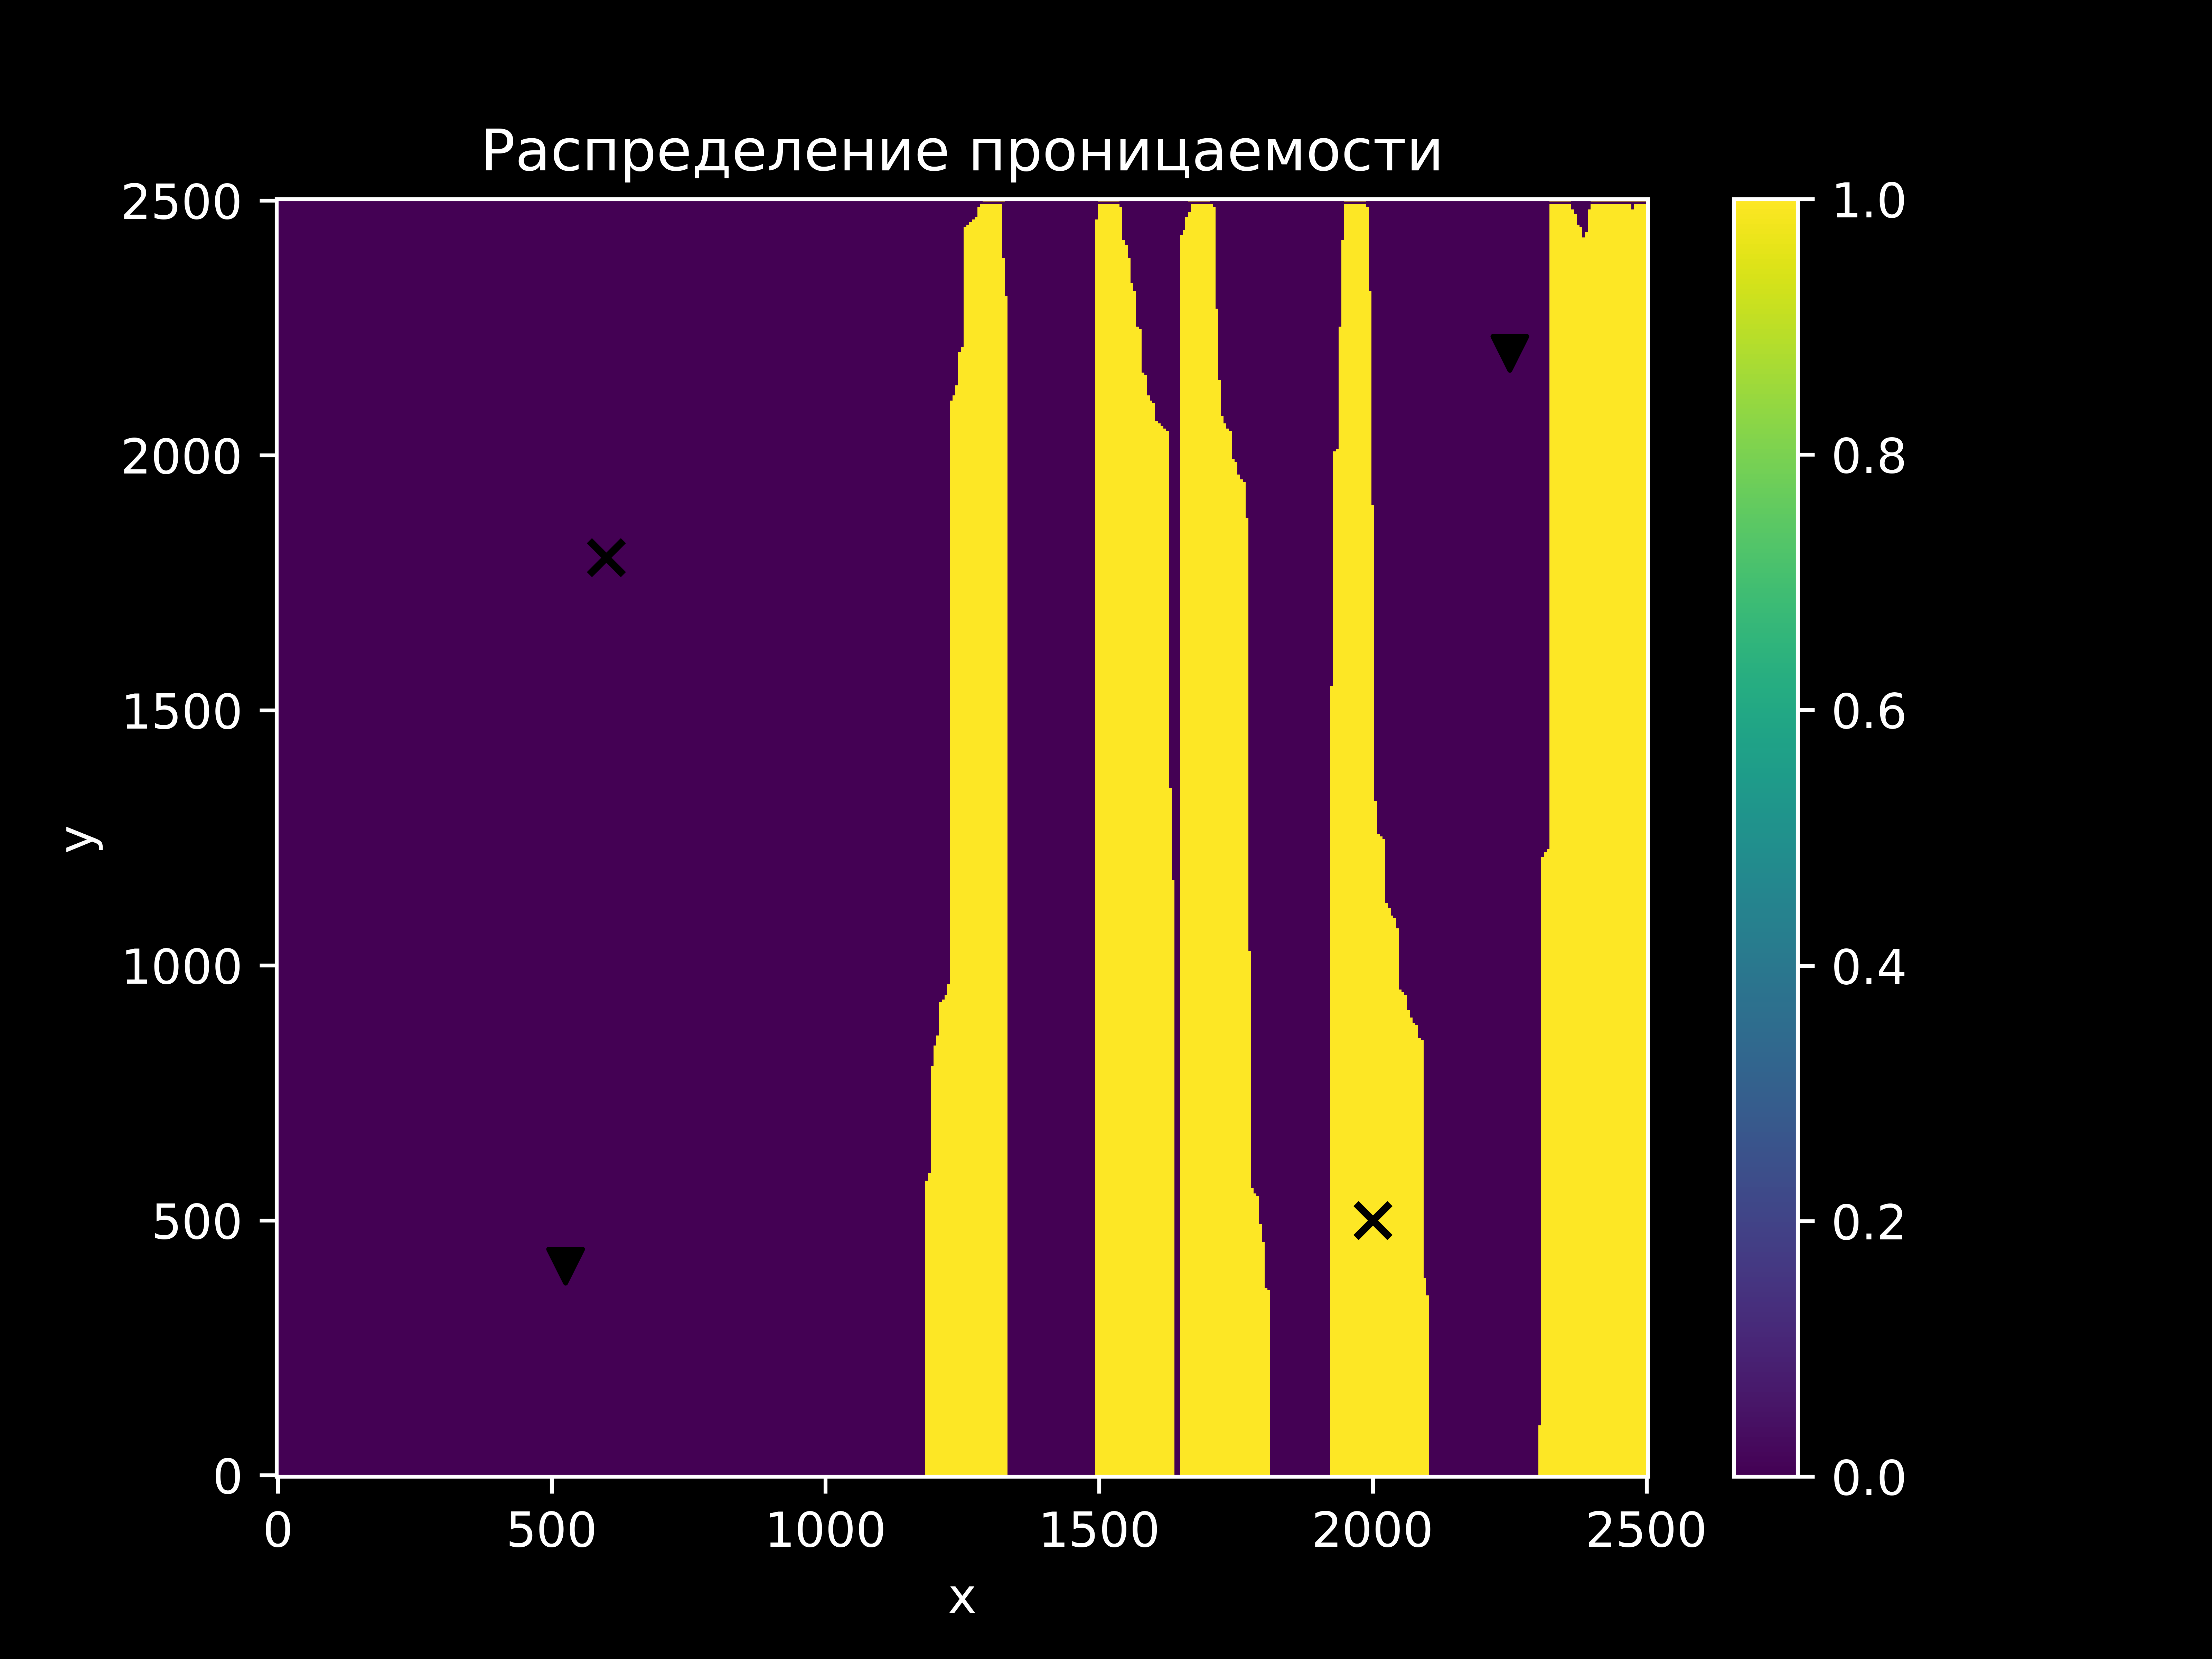
\includegraphics[width=1.0\textwidth]{проницаемость.png}
    \caption{Пример проницаемости пласта}
\end{figure}

\begin{figure}[h]
    \centering
    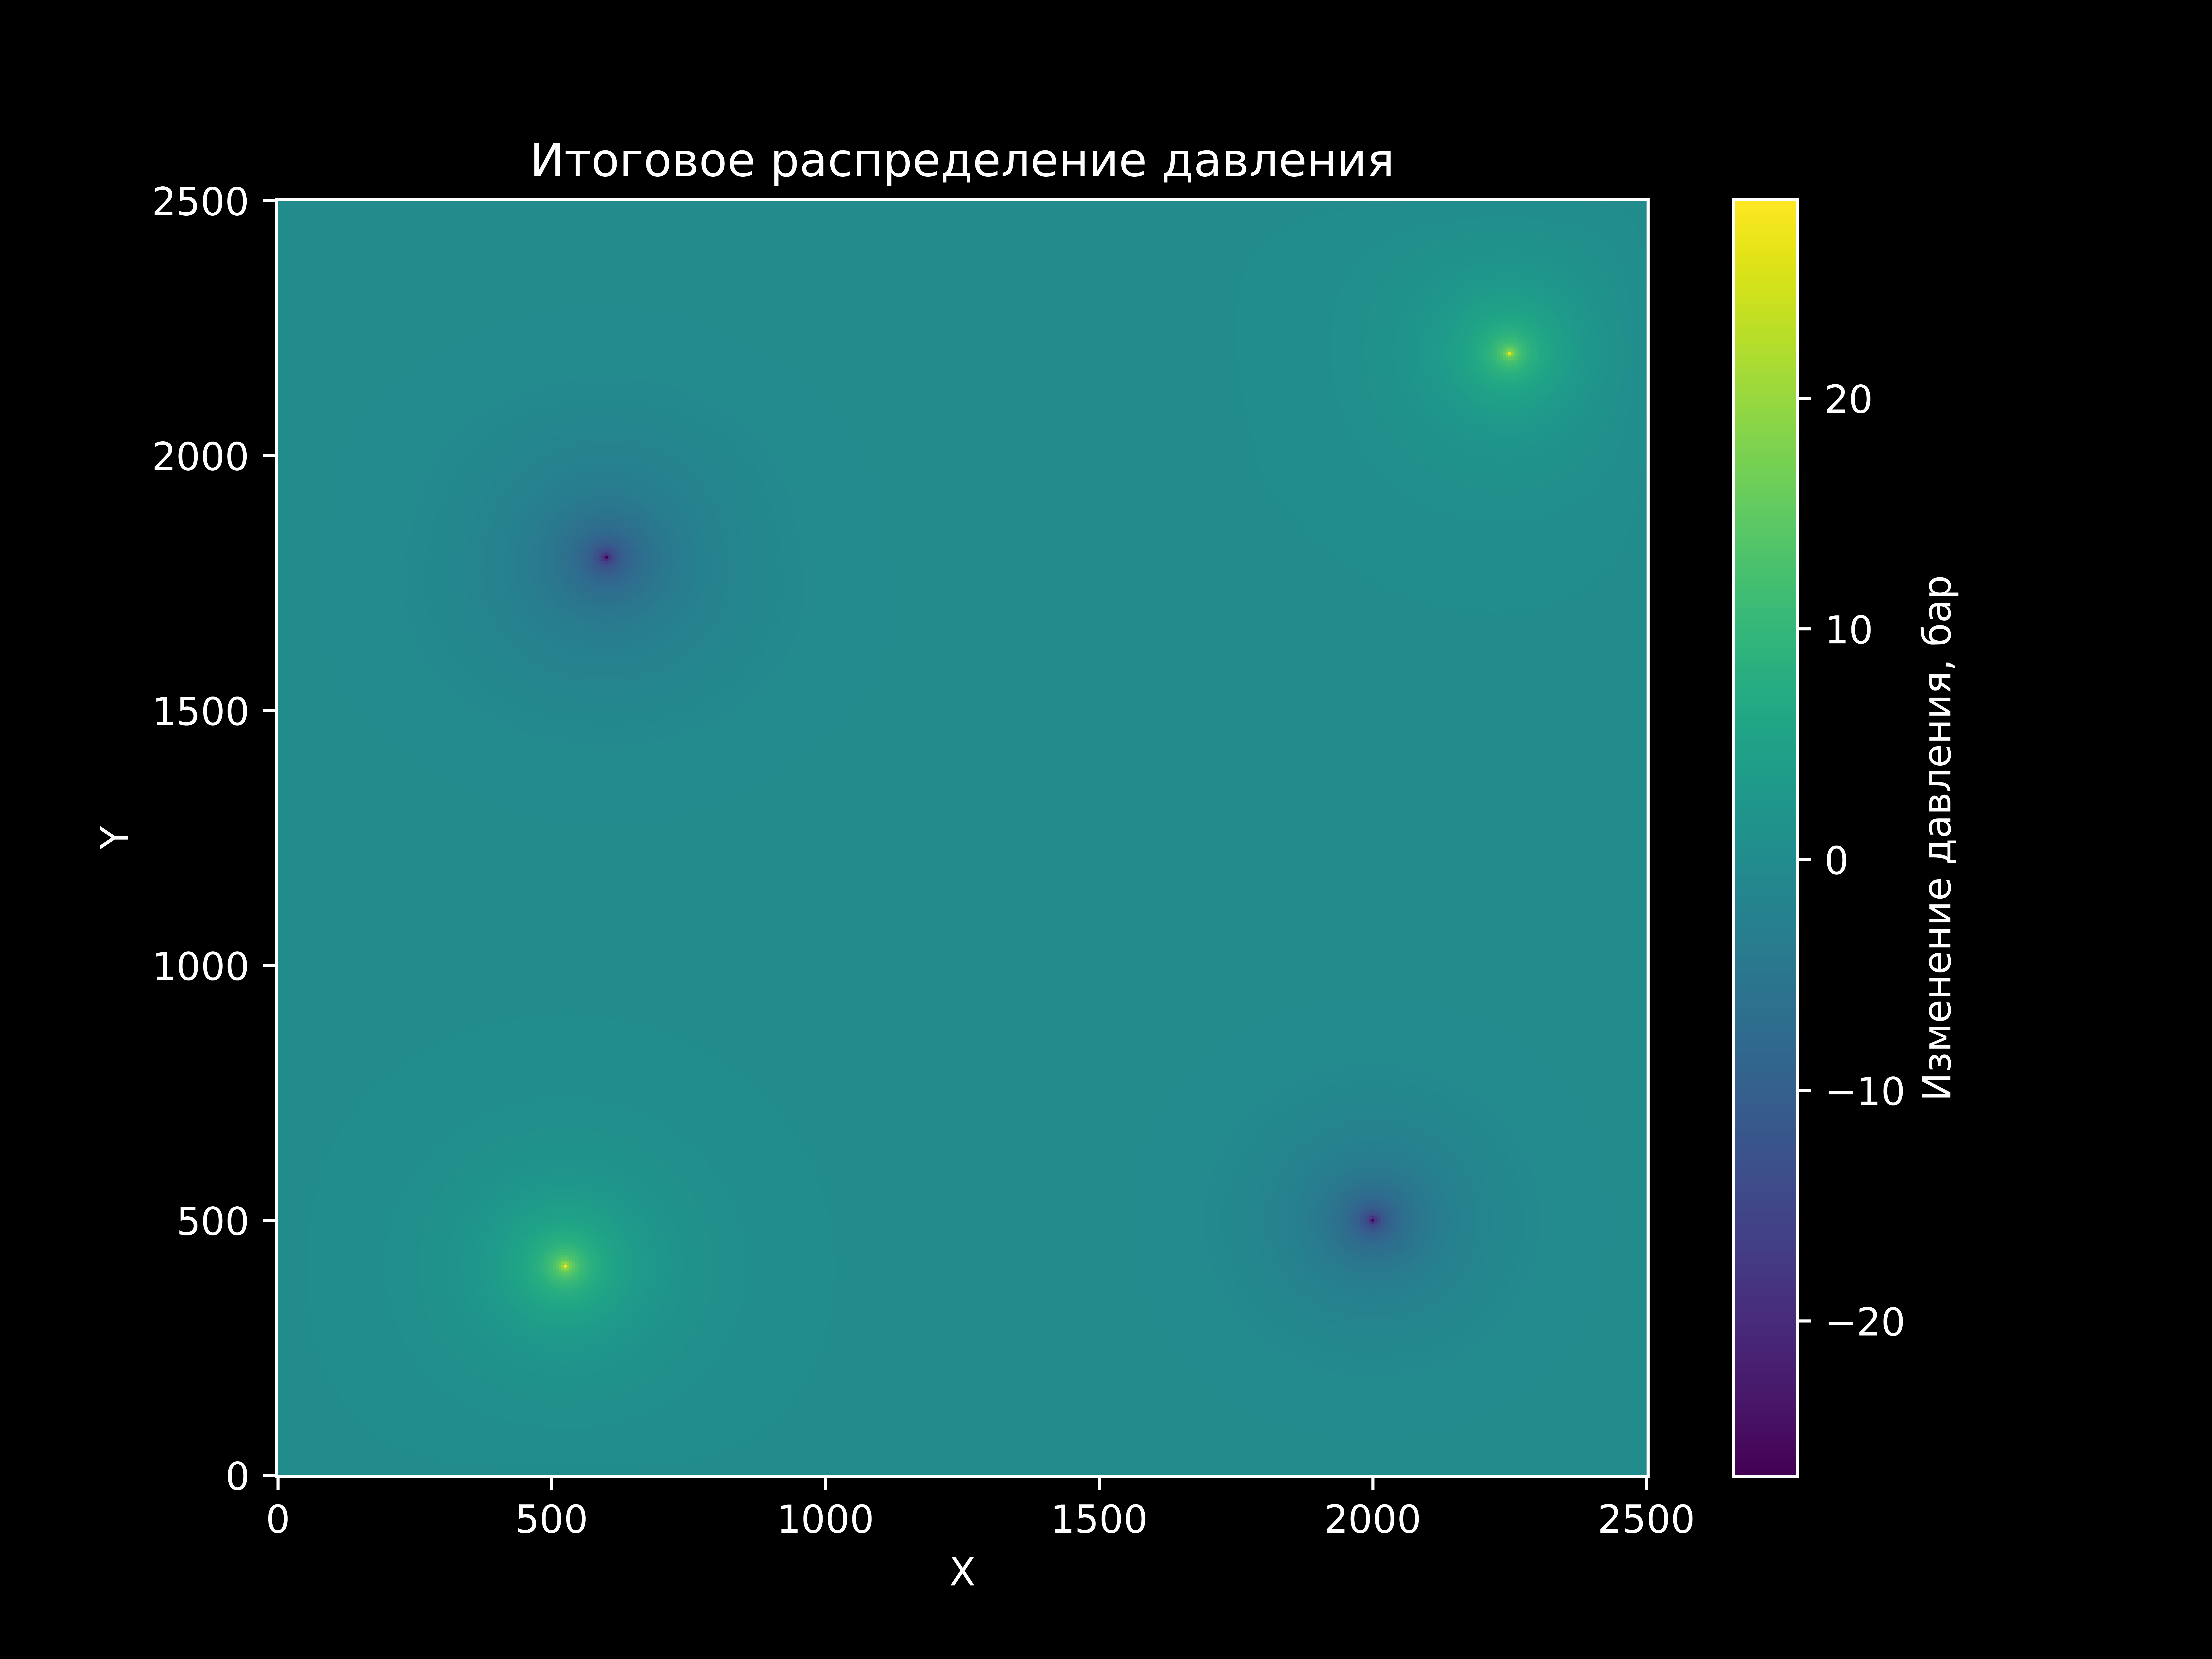
\includegraphics[width=1.0\textwidth]{результат_давление.png}
    \caption{Пример результирующего давления в пласте}
\end{figure}

\begin{figure}[h]
    \centering
    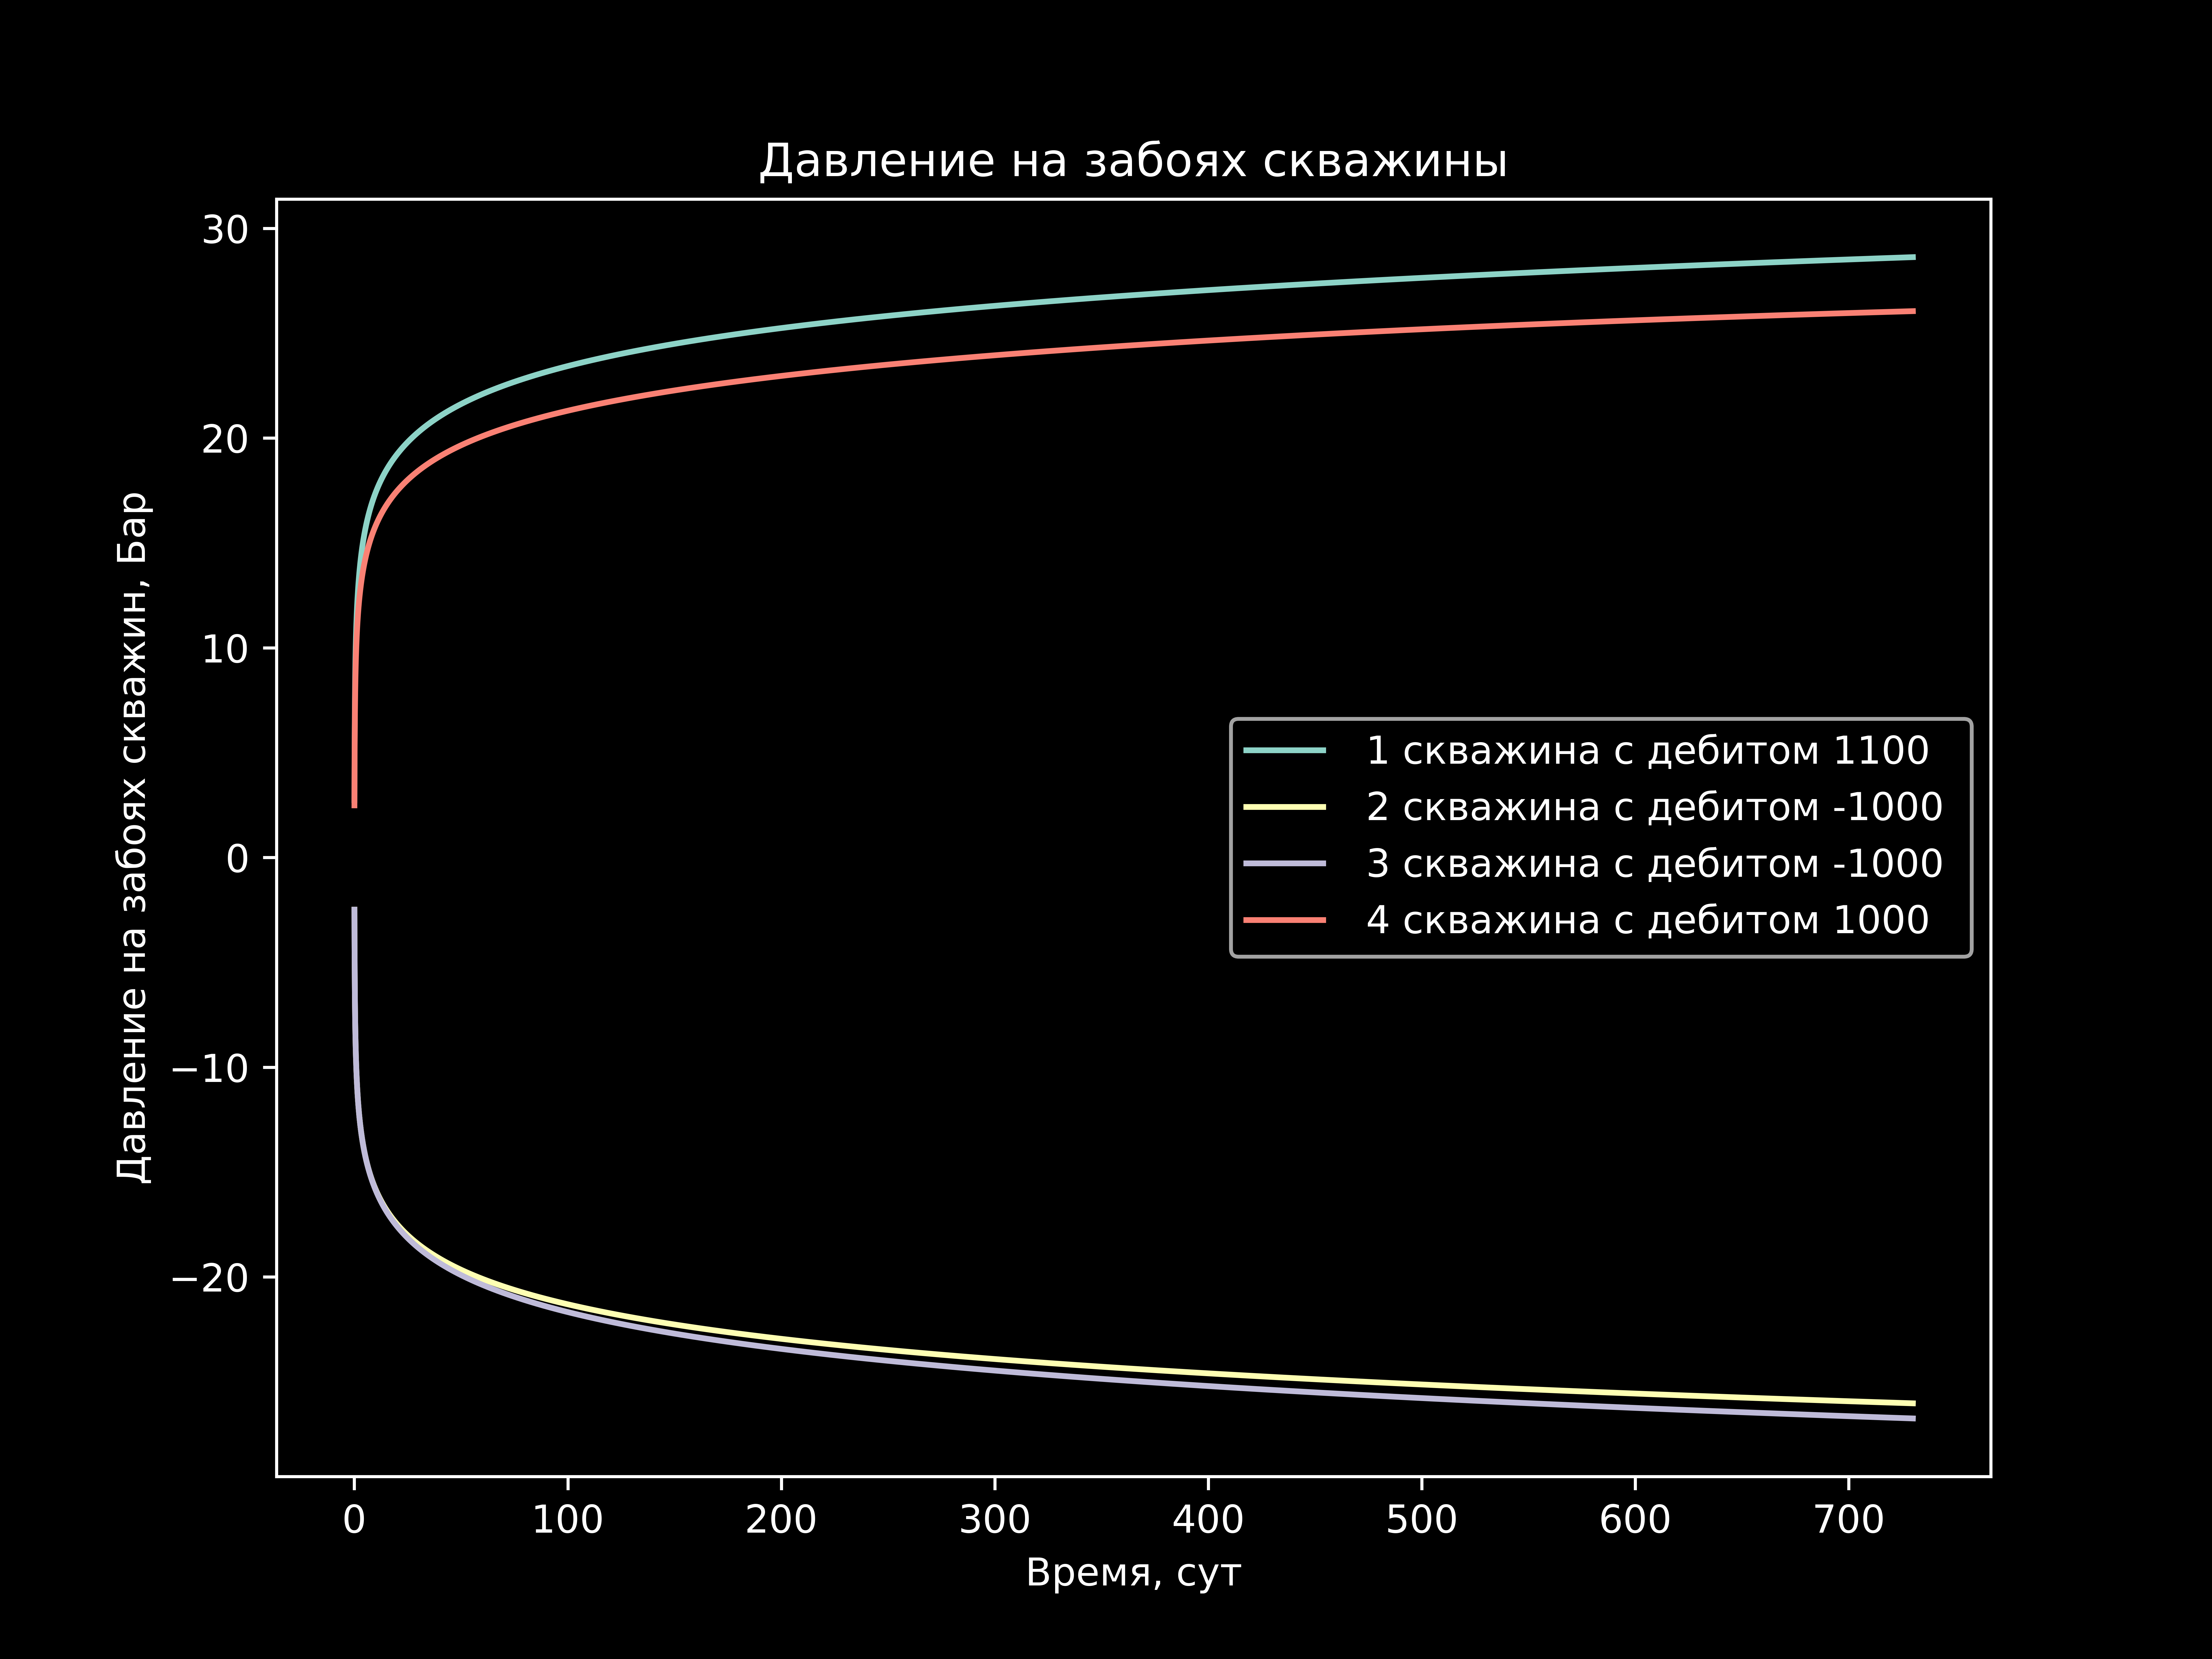
\includegraphics[width=1.0\textwidth]{давление_забой.png}
    \caption{Пример давлений на забоях скважин}
\end{figure}

\begin{figure}[h]
    \centering
    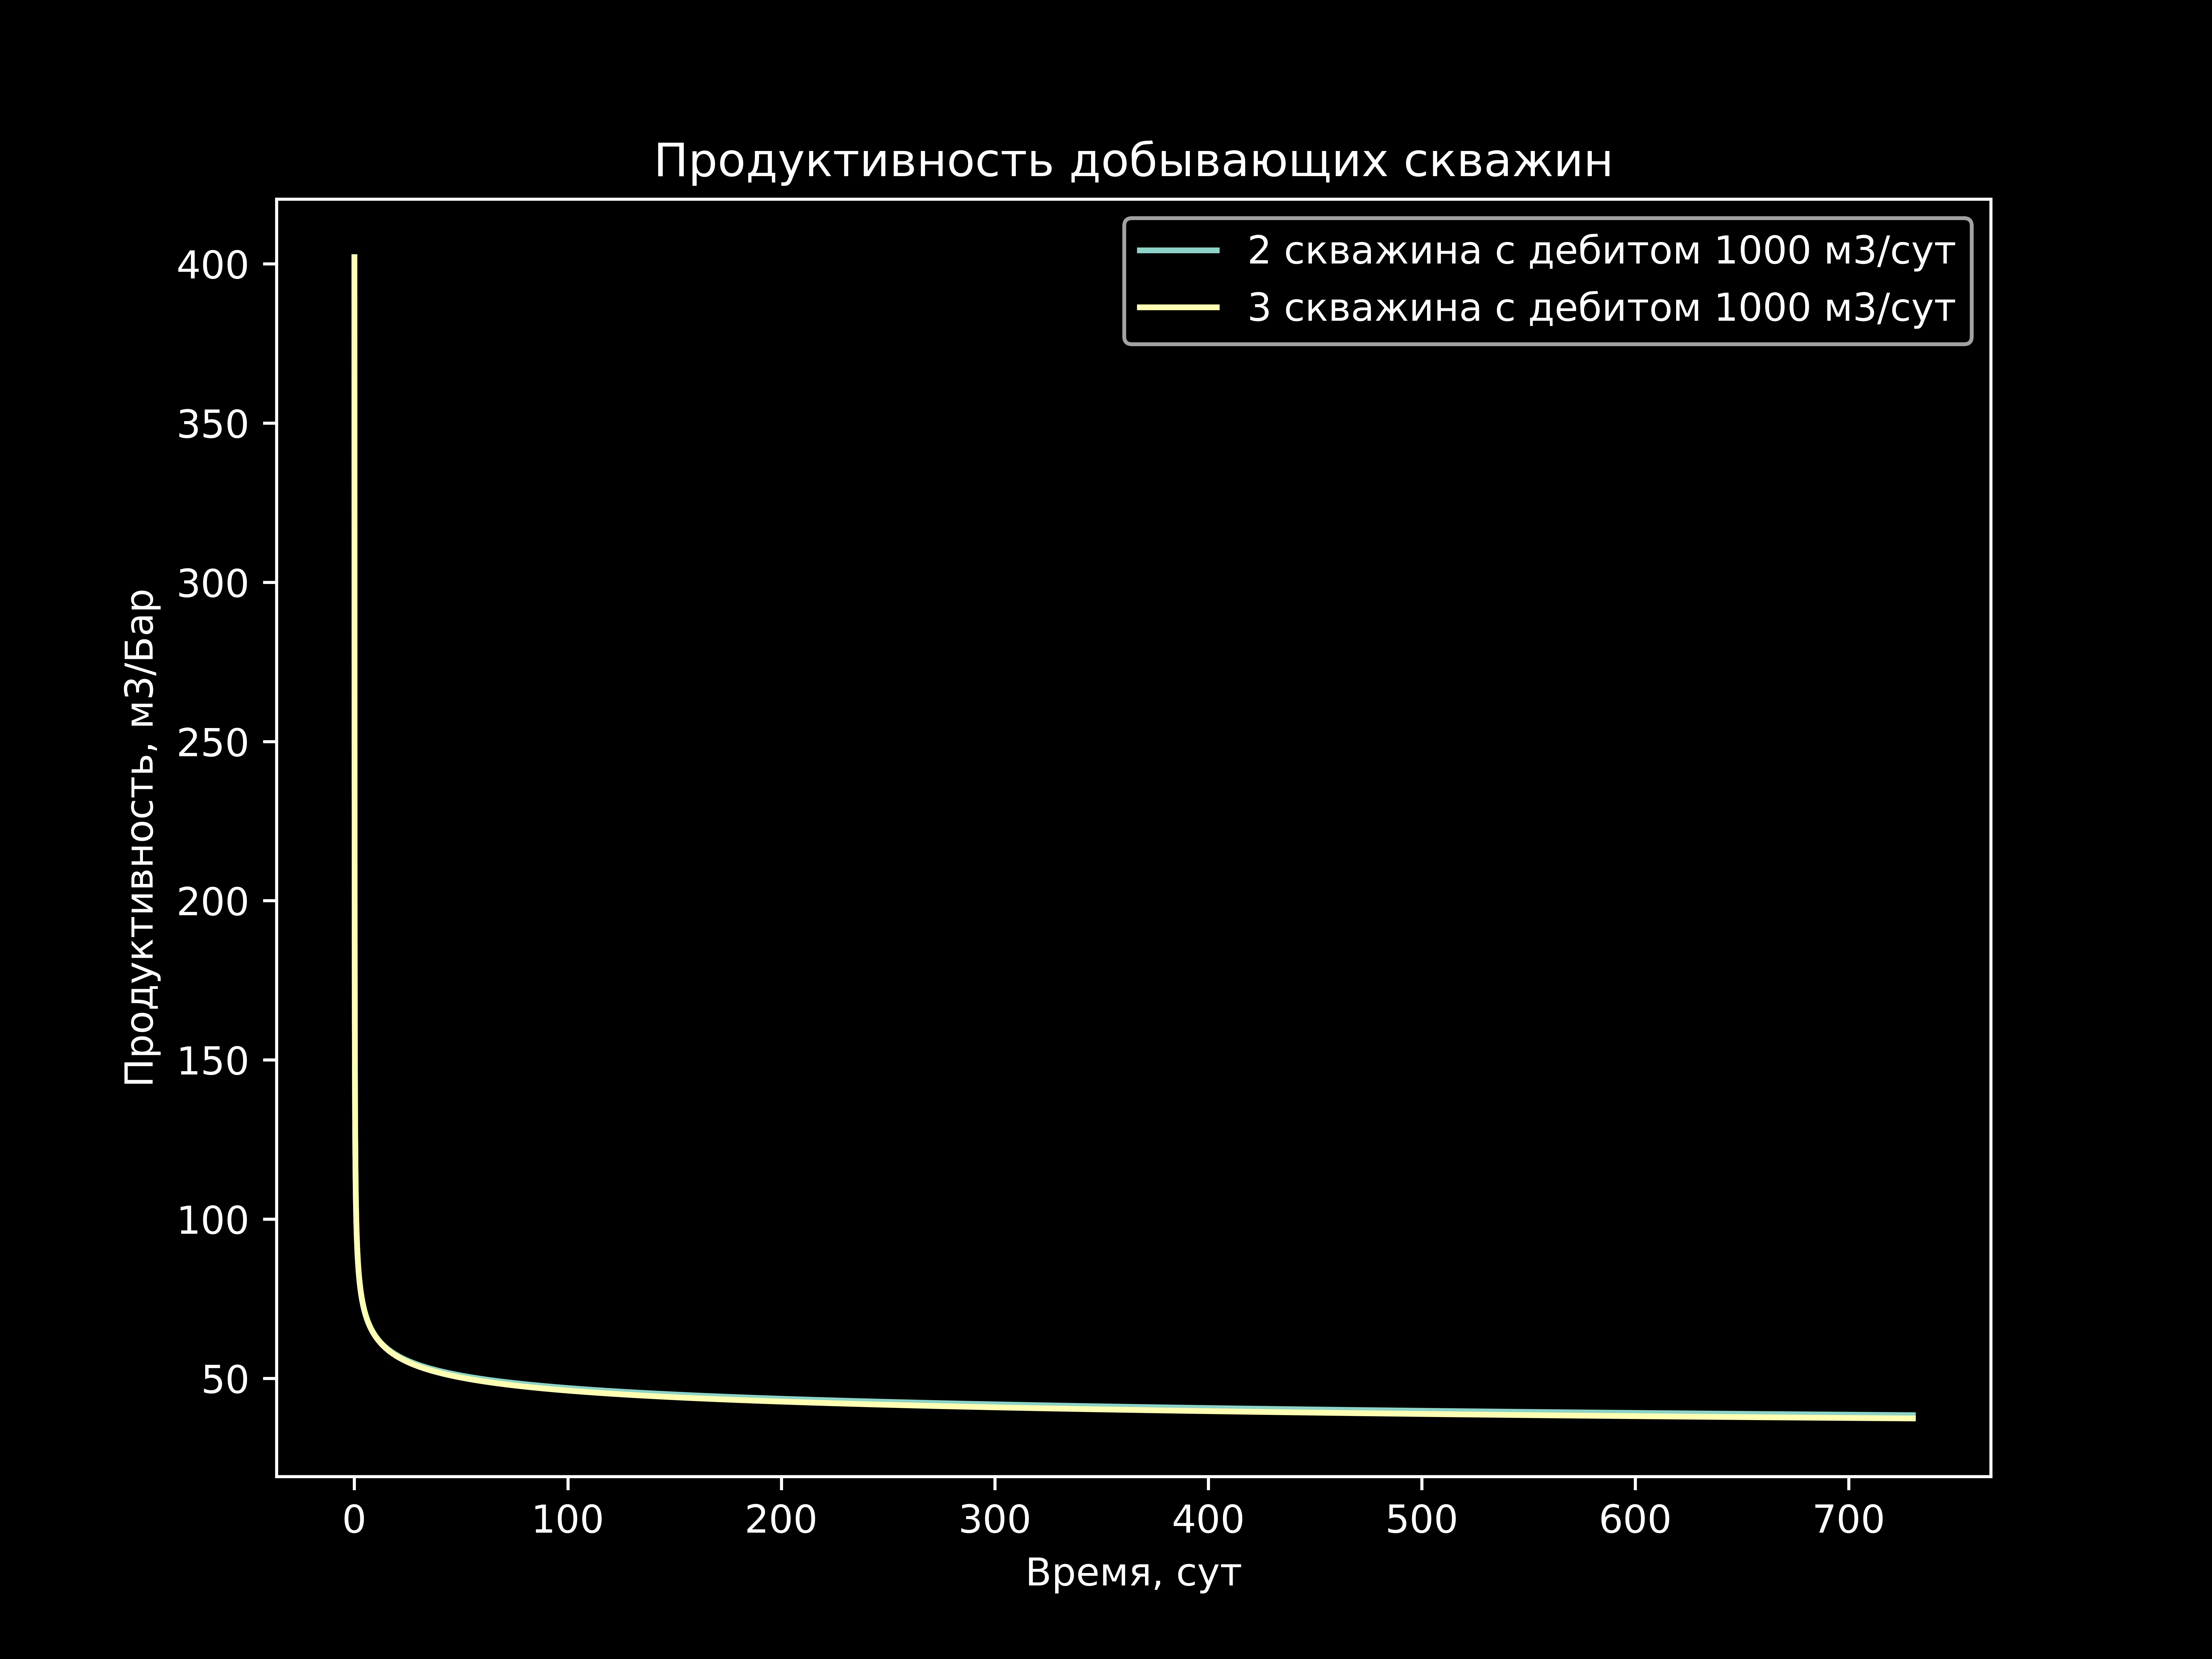
\includegraphics[width=1.0\textwidth]{продуктивность.png}
    \caption{Пример продуктивностей}
\end{figure}





\end{document}